\documentclass[tikz,border=20pt]{standalone}
\usetikzlibrary{calc}

\begin{document}
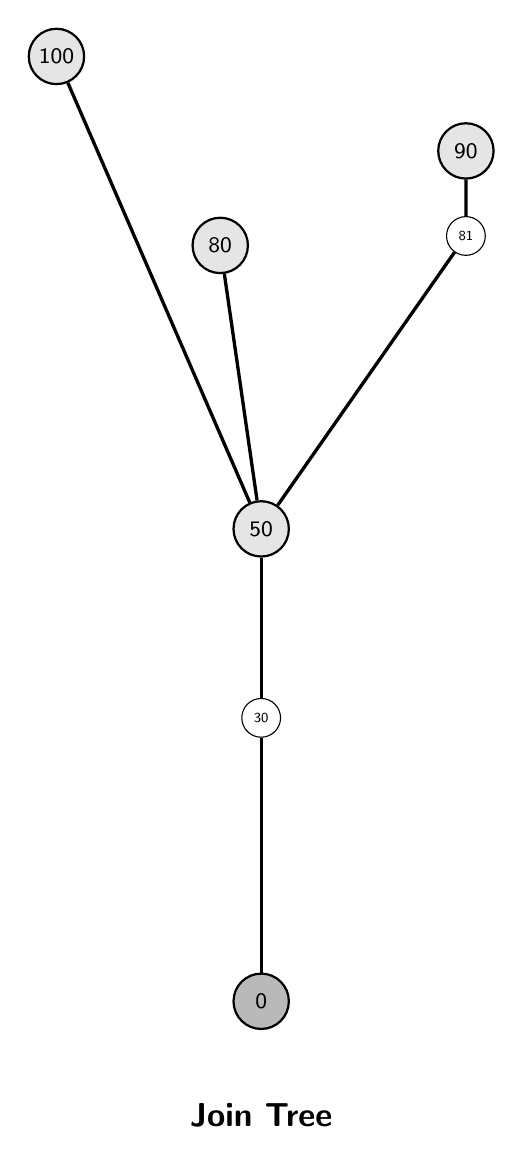
\begin{tikzpicture}[
    y=0.12cm, x=2.6cm,
    crit node/.style={circle, draw=black, fill=gray!20, thick, inner sep=1pt, minimum size=20pt, font=\sffamily\footnotesize},
    min node/.style={circle, draw=black, fill=gray!55, thick, inner sep=1pt, minimum size=20pt, font=\sffamily\footnotesize},
    reg node/.style={circle, draw=black, fill=white, inner sep=0.5pt, minimum size=14pt, font=\sffamily\tiny},
    main edge/.style={very thick, draw=black}
]

% Join Tree: 自上而下追踪超水平集 {f>=h} 的合并
% 关键点 = 极大值 (100,90,80) + join 鞍点 (50); 根 = 全局极小 (0)
% 退化为正则点: split 鞍点 81、30；局部极小 71、20 被剪枝
\node[crit node] (J100) at (0.0, 100) {100};
\node[crit node] (J80)  at (0.8,  80) {80};
\node[crit node] (J90)  at (2.0,  90) {90};
\node[reg  node] (J81)  at (2.0,  81) {81};
\node[crit node] (J50)  at (1.0,  50) {50};
\node[reg  node] (J30)  at (1.0,  30) {30};
\node[min  node] (J0)   at (1.0,   0) {0};

% join 鞍点 50: 极大值 100、80 与 90 (经正则点 81) 三分量在此合并
\draw[main edge] (J100) -- (J50);
\draw[main edge] (J80)  -- (J50);
\draw[main edge] (J90)  -- (J81) -- (J50);

% 主干下行至全局极小 0 (途经正则点 30)
\draw[main edge] (J50) -- (J30) -- (J0);

\node[font=\sffamily\bfseries\large] at (1, -12) {Join Tree};

\end{tikzpicture}
\end{document}
